% !TeX root = ../main.tex

\chapter{Software}\label{chapter:Software}

This chapter gives an overview of software used to implement this thesis.


\section{Neurorobotics Platform}\label{section:NeuroroboticsPlatform}

The \textit{\gls{nrpa}} is a subproject of the \textit{Human Brain Project}\footnote{The Human Brain Project is a large 10 year scientific project funded by the European Union \enquote{building a research infrastructure to help advance neuroscience, medicine and computing} \autocite{hbpOverview}} which \enquote{allows researchers to give any simulated brain model its own 'body' — virtual or even real — and explore how it controls movement, reacts to stimulus and learns in a virtual environment} \autocite{neuroroboticsOverview}.
\newline
One application of this is to assess the fidelity of a certain brain simulation, under the assumption that a combination of body and simulated brain behaving similarly to its real counterpart would validate the brain simulation \autocite{neuroroboticsOverview}. The project is creating a complete virtual mouse, which will have all the same sensory organs as well as bones and muscles made to mimic their counterparts in a real mouse. The aim is to be able to use this mouse in virtual experiments, with the added benefit of monitoring the simulated brain in real-time for analysis, as well as to perform experiments which are impractical in the real world due to their scope, since practically all data of the simulation can be recorded and the simulation sped up by orders of magnitude \autocite{neuroroboticsVision}. Another intended use case is for the development of robots. The \textit{\gls{nrpa}} allows robots to be quickly and reliably created and tested in a virtual environment, prior to an actual prototype being been built \autocite{neuroroboticsOverview}.
\newline

The backend of the \textit{\gls{nrpa}} is intended to be run independently from the frontend, for example on a high performance server. The user connects to it via a web frontend, which is called the \textit{web cockpit} (see \autoref{fig:NRPWebCockpit}), with a supported browser, where he can choose from a list of premade experiments, or create his own.
\begin{figure} [h]
    \centering
    \subfloat[\gls{nrpa} Web Cockpit]{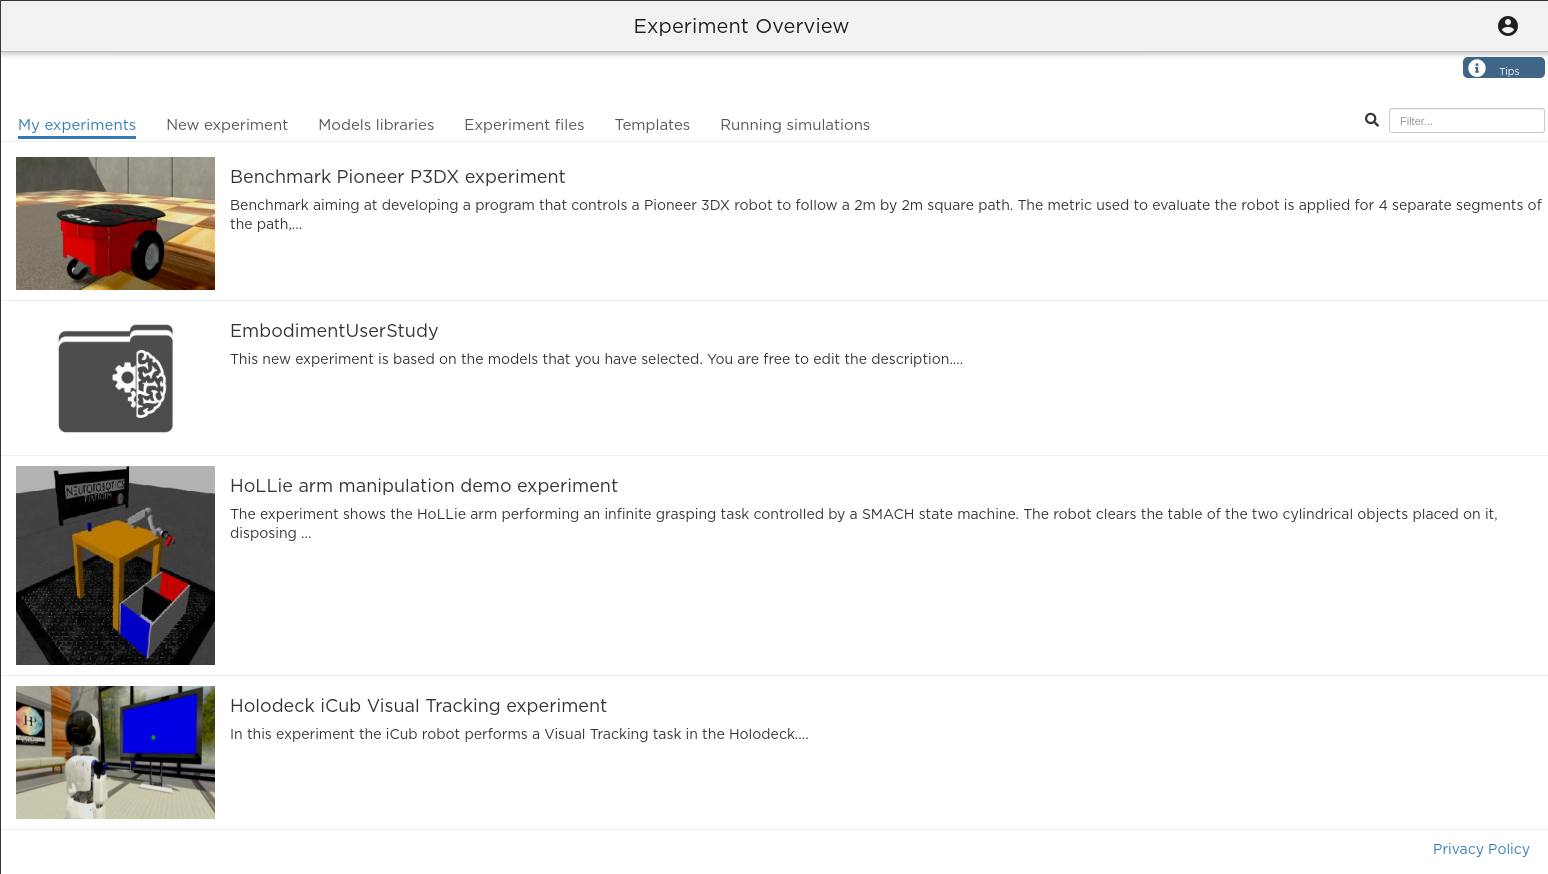
\includegraphics[width=0.48\textwidth]{figures/NRPCockpit}\label{fig:NRPWebCockpit}}
    \hfill
    \subfloat[\gls{nrpa} Simulation View]{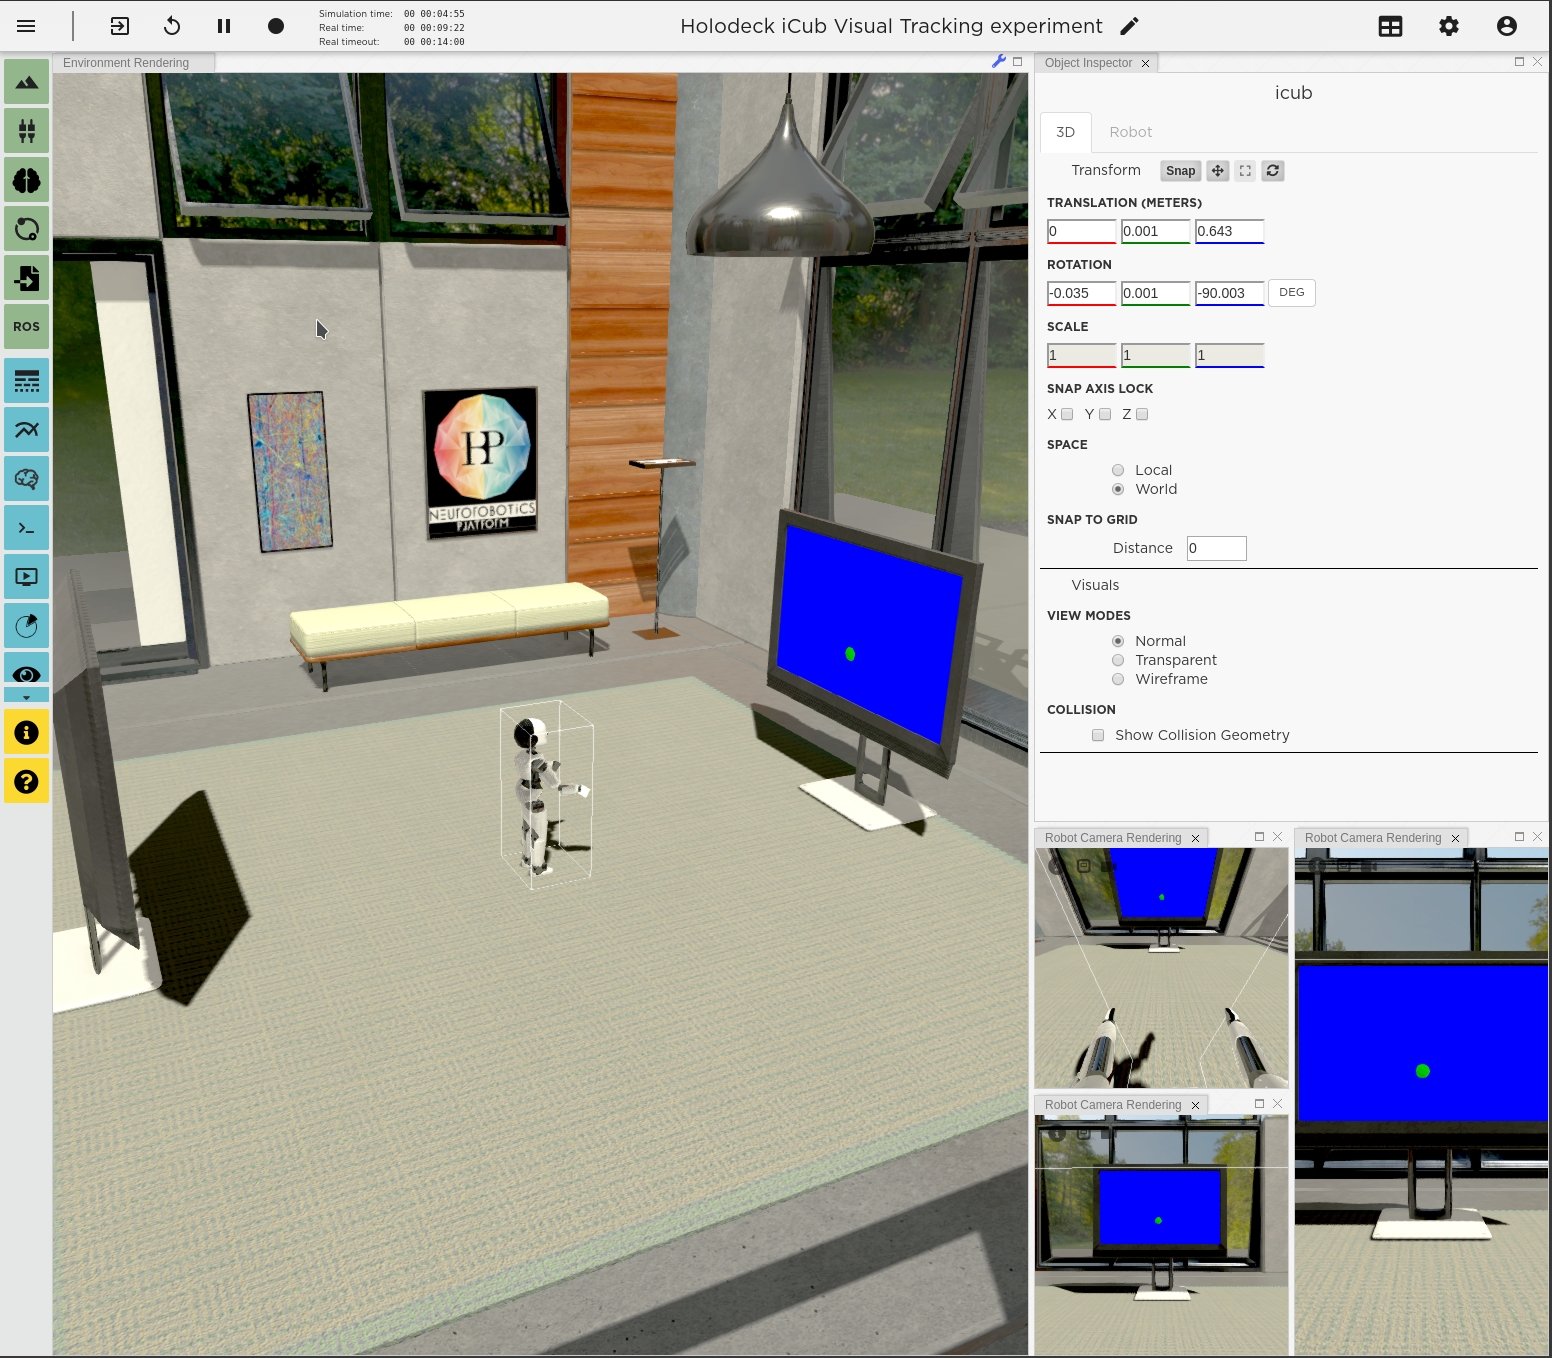
\includegraphics[width=0.48\textwidth]{figures/NRPSimulationView}\label{fig:NRPSimulationView}}
    \caption{\gls{nrpa} Frontend}
    \label{fig:NRPFrontend}
\end{figure}
Once a simulation is started, the user is presented with the \textit{simulation view} (see \autoref{fig:NRPSimulationView}) in which he can pause, inspect and manipulate the experiment. The camera can be freely moved, objects can be teleported elsewhere or have forces applied to them interactively, and the state of the experiment, for example visual input the robot recieves, can be viewed in real time.
\newline
Only the graphics are rendered locally on the user's machine, the heavy computations of the rest of the simulation are all done by the backend, potentially on another machine.


\section{Unity3D with SteamVR}

\textit{Unity3D} is a cross-platform game engine that was originally launched exclusively for \textit{Mac OS-X} in 2005 \autocite{unityAt10}, but has since been expanded to support most desktop operating systems, consoles, mobile devices, web browsers, and most \gls{vra} and \gls{ara} platforms, a total of more than 25 platforms. It is continually being developed by \textit{Unity Technologies}, and is available gratis for personal use \autocite{unity}.
\newline
More than half of all mobile games, as well as 60\% of \gls{vra} and \gls{ara} content is created with \textit{Unity3D} \autocite{deepMindPartner}.
\newline

\textit{SteamVR} is a \gls{vra} platform developed by \textit{Valve Inc.} originally for the \textit{HTC Vive} (see \autoref{chapter:Hardware}) that implements the \textit{OpenVR} \gls{apia} \enquote{that acts as the interface between VR hardware and software}, which makes it compatible with any headset that supports \textit{OpenVR} \autocite{steamVRArticle}.
\newline
\textit{SteamVR} is available as a plugin for \textit{Unity3D}, allowing for easy integration of \textit{HTC Vive} hardware into any project.



\section{Neurorobotics Unity3D Client}\label{section:NeuroroboticsUnity3DClient}

The \textit{Neurorobotics Unity3D Client} (referred to as client from here on) is a \gls{vra} client for the \gls{nrpa}. At the time of writing, it connects to a running simulation on the \gls{nrpa}, from which it receives the entire scene information, meaning the position of all objects in the simulation. The client does not handle any of the physics calculations, the client only gets updated scene information from the \gls{nrpa} instance to which it is connected.
\newline
In addition to displaying the simulation, the client can spawn a humanoid body for the user (referred to as avatar from here on).
\newline 
This initially takes the shape of a translucent avatar, which follows the tracked position of the user without colliding with any objects of the simulation on the \gls{nrpa}, and is referred to as the \textit{local} avatar. The local avatar is only present in the client. It is implemented using \textit{Unity3D}'s animation system, which includes special features for humanoid characters. Target positions for hands, feet, head and body can be set, after which the animation system will calculate a joint configuration to match these target positions using \gls{ika}, and animate the avatar according to changing targets.
\newline
A corresponding avatar is spawned on the \gls{nrpa} instance, appearing as an opaque copy of the local avatar. This \textit{remote} avatar is a robot, which will try to achieve the same pose as the local avatar, but while doing so will be constrained by the physics of the \gls{nrpa}.

\begin{figure}[h]
    \centering
    \subfloat[Translucent local avatar only]{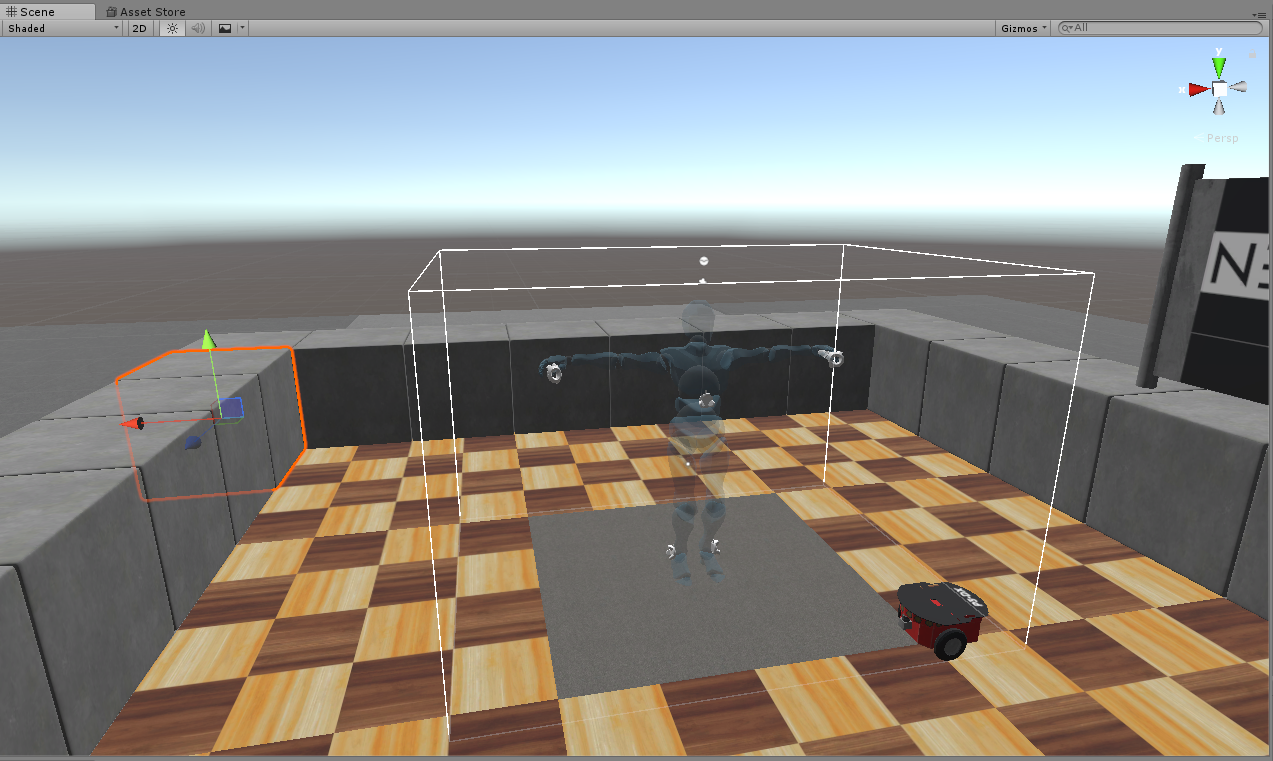
\includegraphics[width=0.48\textwidth]{figures/UnityClientLocalAvatar}\label{fig:unityClientLocalAvatar}}
    \hfill
    \subfloat[Opaque remote avatar spawned in]{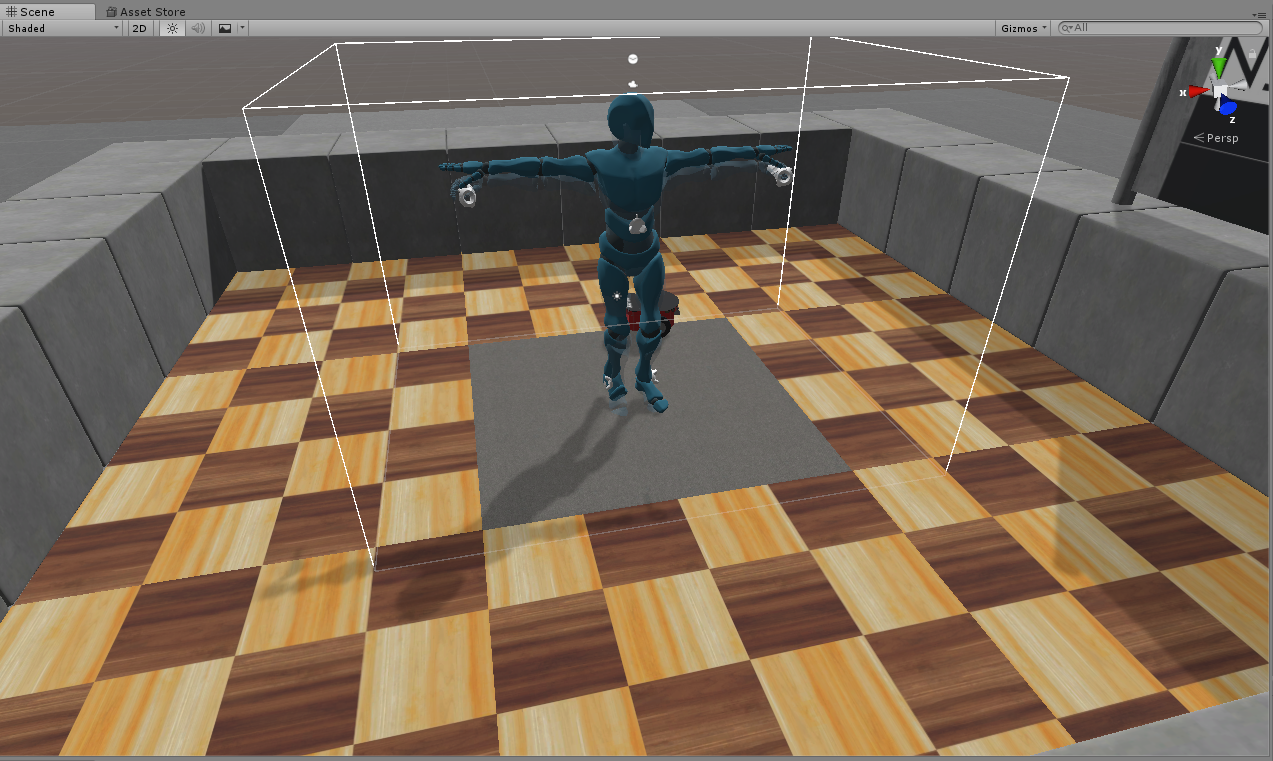
\includegraphics[width=0.48\textwidth]{figures/UnityClientRemoteAvatar}\label{fig:unityClientRemoteAvatar}}
    \caption{Simulation as seen in Unity3D client, with local and remote avatars}
    \label{fig:unityClientLocalRemote}
\end{figure}

The base state of the client was easily extendable to include full body tracking by adding three \textit{Vive Trackers} (see \autoref{chapter:Hardware}) to the scene, and assigning them to the corresponding animation targets of the local avatar. 
\newline
With this modification, the user is able to navigate the play space (shown as a box with white borders) in the virtual environment on the \gls{nrpa} with a fully tracked body.